\documentclass{beamer}
\usetheme{Madrid}
\definecolor{feadevcolor}{rgb}{0.96, 0.902, 0.027}
\definecolor{nodecolor}{rgb}{0.478, 0.451, 0.012}
\usecolortheme[named=feadevcolor]{structure}

\usepackage[utf8]{inputenc}
\usepackage{tikz, pgfplots}
\usepackage{amsmath, amsthm, amsfonts, amssymb, dsfont, mathtools}
\usepackage{minted}
\usepackage{listings}
\usepackage{array, makecell}
\usepackage{fontawesome}
\renewcommand\theadfont{\bfseries}
\setbeamertemplate{caption}[numbered]{}
\usetikzlibrary{trees}

\tikzset{noo/.style={circle, draw=nodecolor, fill=nodecolor, minimum size=0.5cm}}

\tikzset{leafs/.style={circle, draw=feadevcolor, fill=feadevcolor, minimum size=0.5cm}}

\tikzset{arrowstart/.style={->}}


\title{\textbf{Tree-Based Methods}}
\subtitle{Statistical Learning}
\author[FEA.dev]{Douglas Cardoso}
\institute[]{FEA.dev - Inteligência Artificial}
\date{April 2021}

\pgfplotsset{compat=1.17} % foi pedido pelo programa

\hypersetup{pdfpagemode=FullScreen}
\begin{document}
    \begin{frame}
    \titlepage
    \end{frame}
    
\AtBeginSection[]
{
  \begin{frame}
    \frametitle{Table of Contents}
    \tableofcontents[currentsection]
  \end{frame}
}
 
\section{Generalization Error}
\begin{frame}{Estimação da função $f$}

\begin{block}{Por que estimar $f$?}
    Podemos querer estimar $f$ por dois motivos principais: \textbf{inferência} e \textbf{predição}. Em predição, o objetivo é encontrar $\hat{f}$ tal que $\hat{f} \approx f$.
\end{block}

Dado $p$ preditores diferentes $X_1, X_2, ..., X_p$, assumimos que há  uma relação entre $Y$ e $X$, que pode ser escrita como
    
    \begin{equation}
        Y = f(x) + \epsilon
    \end{equation} 
    
onde, $f(x)$ é uma função desconhecida e $\epsilon$ é um \textit{random error term} (com média aproximadamente zero). E tentamos prever $Y$ usando,

\begin{equation}
        \hat{Y} = \hat{f}(x)
    \end{equation}
    
em que, $\hat{f}$ é uma estimativa de $f$ e $\hat{Y}$ é o resultado da predição para $Y$.
\end{frame}

\begin{frame}{Tipos de erros}

A acurácia de $\hat{Y}$ depende de dois tipos de erros, do qual a minimização do segundo será o nosso foco:

\begin{columns}
    \column{.45\linewidth}
    \begin{block}{Reducible Error}
        \small Erros introduzidos pela estimativa \textit{naturalmente} imperfeita de $\hat{f}$ para $f$, que podem ser reduzidos com algumas medidas de aprimoramento do modelo
    \end{block}
    \column{.45\linewidth}
    
    \begin{block}{Irreducible Error}
        \small Erros que não podem ser previstos usando $X_p$, afetam a acurácia da nossa predição e sua existência se deve a variáveis e variações não mensuradas nos dados.
    \end{block}
\end{columns}
\vspace{0.05\linewidth}

Formalmente, temos esses erros representados na média quadrática da diferença entre $\hat{Y}$ e $Y$, definida por

\begin{equation}
    \mathbf{E}(\mathbf{Y}- \hat{\mathbf{Y}}) = \mathbf{E}[f(x) + \epsilon - \hat{f}(x)]^2 = 
    \underbrace{[f(x) - \hat{f}(x)]^2}_\text{reducible} + \overbrace{Var(\epsilon)}^{\text{irreducible}}
\end{equation}

\end{frame}

\begin{frame}{Medida de qualidade dos ajustes modelísticos}

\begin{block}{Para regressão}
    A maneira mais usada para medir a performance do nosso modelo de regressão é o  \textit{mean squared error} (MSE), dado por
    
    \begin{equation}
        MSE = \frac{1}{n} \sum_{i=1}^{n} (y_i - \hat{f}(x_i))^2
    \end{equation}
    MSE é computado usando \textit{training data}, então por isso chamamos de \textbf{\textit{training MSE}}. Mas, em geral, não estamos interessados se $\hat{y}(x_i) \approx y_i$ e sim se $\hat{y}(x_0) \approx y_0$, onde $(x_0, y_0)$ são dados de testes não incorporados no treinamento do modelo. Então nos importa mais o \textbf{\textit{test MSE}}:
    
    \begin{equation}
        Ave(\hat{f}(x_0) - y_0)^2
    \end{equation}
 \vfill
 
\end{block}

    
\end{frame}

\begin{frame}{Medida de qualidade dos ajustes modelísticos}
    \begin{block}{Para classificação}
        Em modelos de classificação, a abordagem mais comum é a proporção de erros cometidos por nosso modelo $\hat{f}$, chamado de \textit{training error rate}:
        
        \begin{equation}
            \frac{1}{n} \sum_{i=1}^n I(y_i \neq \hat{y}_i)
        \end{equation}
        
        E o \textit{test error rate}, associado com as observações de testes é definido por
        
        \begin{equation}
            Ave (I(y_0 \neq \hat{y}_0),
        \end{equation}
        em que $\hat{y}_0$ é o \textit{class label} previsto para o preditor $x_0$.
        \vfill
    \end{block}
\end{frame}

\begin{frame}{Test MSE Decomposition}
Podemos decompor o \textit{expected test MSE} em três partes:
\begin{equation}
    E(y_0 - \hat{f}(x_0))^2 = Var(\hat{f}(x_0)) + [Bias(\hat{f}(x_0))]^2 + Var(\epsilon)
\end{equation}
Isso nos diz que para minimizarmos o MSE, precisamos de um modelo com uma \textbf{baixa variância} e \textbf{baixo viés}. Afinal, o que significam esses termos?

    \begin{block}{Variance}
        Valor pelo qual $\hat{f}$ muda se o estimamos usando um conjunto de dados de treinamento diferente.
        \begin{itemize}
            \item Modelos mais flexíveis têm variâncias mais alta;
            \item Pequenas modificações no conjunto de treino pode resultar em grandes alterações em $\hat{f}$.
        \end{itemize}
    \end{block}
    
     \begin{block}{Bias (Viés)}
        O quando nossa estimativa de $f$ difere de $f$, isto é, o quanto $\hat{f} \neq f $.
        
        \begin{itemize}
            \item Modelos mais flexíveis têm menos viés.
        \end{itemize}
    \end{block}

\end{frame}

\begin{frame}{Model flexibility e Bias-Variance Tradeoff}
\begin{alertblock}{Overfitting}
 \textit{Small training MSE, Large test MSE}
 
\end{alertblock}
    \begin{figure}
        \centering
        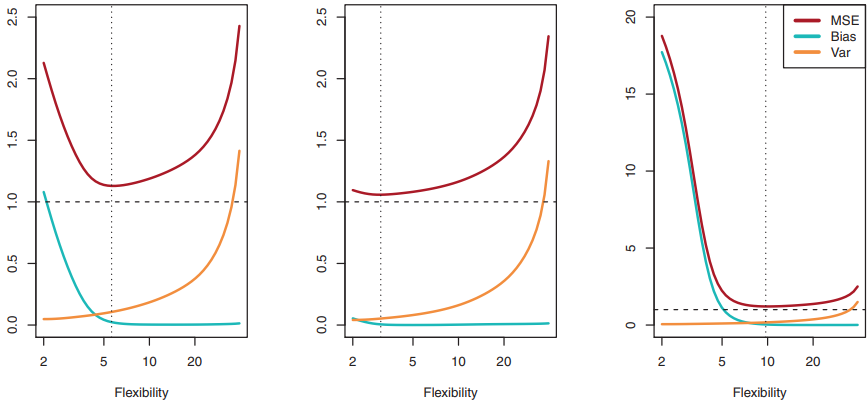
\includegraphics[height=5cm]{pic/mse_bias_var.png}
        \caption{\scriptsize \textit{Squared bias (blue curve), variance (orange curve), Var($\epsilon$) (dashed line), and test MSE (red curve). The vertical dotted line indicates the flexibility level corresponding to the smallest test MSE.}}
        \label{fig:my_label}
    \end{figure}
\end{frame}
\section{O que são árvores?}

    \begin{frame}[t]{Árvores}
    \vspace{1em}
    \begin{block}{Definição}
        É um grafo conexo, acíclico onde um dos vértices é diferenciado dos deamis, organizando os dados em um conjunto de \textbf{registros que satisfaz certas condições}.
    \end{block} \vspace{1.5em}
        \begin{itemize}
            \item Registros serão chamados de \textbf{nós} (node);
            \item O nó por qual conseguimos acessar qualquer outro nó, é chamado de \textbf{raiz} (root);
            \item O nó que não tem ancestralidade de outros nós, é chamado de \textbf{folha} (leaf).
        \end{itemize}
    \end{frame}

\begin{frame}[t]{Árvore de decisão}
\vspace{1em}
    \begin{block}{Definição}
        Metodologia de representação não paramétrica, supervisionada que leva a resultados facilmente interpretáveis, construída por particionamentos dos espaços recursivamente em retângulos.   
    \end{block}
    \begin{itemize}
        \item Cada particionamento é \textbf{nó};
        \item Cada resultado final é \textbf{folha}.
    \end{itemize}
\end{frame}

\begin{frame}{Representação gráfica de uma árvore}
\begin{figure}
    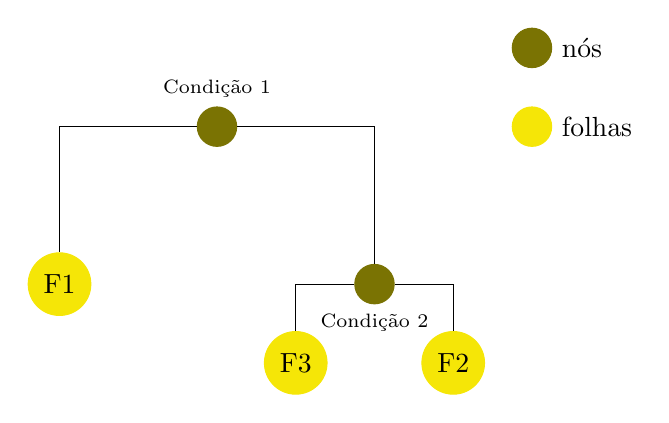
\begin{tikzpicture}
    %[scale=.9,auto=center,every node/.style={circle,fill=blue!20}]
    \node[noo, label=above: \scriptsize{Condição 1}] (a1) at (5,7) {};  
    \node[leafs] (a2) at (3,5) {F1}; 
    \node[noo, label=below: \scriptsize{Condição 2}] (a3) at (7,5) {};  
    \node[leafs] (a4) at (8,4) {F2};  
    \node[leafs] (a5) at (6,4) {F3};  
    
    % legend
    \node[noo, label=right:nós] at (9,8){};
    \node[leafs, label=right:folhas] at (9,7){};
    
    \draw (a1) -| (a2); \pause
    \draw (a1) -| (a3); \pause 
    \draw (a3) -| (a5); \pause 
    \draw (a3) -| (a4); 
    
  
    \end{tikzpicture}
    \caption{Exemplo de estrutura de uma árvore.}
\end{figure}
\end{frame}

\section{A criação de uma árvore de decisão}

\begin{frame}{Criação da estrutura}
\begin{enumerate}
    \item Expansão da árvore: partições no conjunto de treino até que a condição de parada seja satisfeita \textbf{(caso base)};
    
    \vspace{1em}
    
    \item Poda da árvore: reagrumento dos subconjuntos da partição, com finalidade de evitar o overfitting.
\end{enumerate}
\end{frame}

\begin{frame}{Propriedades da expansão da árvore}
\begin{itemize}
    \item As partições são feitas de com cortes ortoganais que maximiza a pureza das sub-regiões resultantes;
    
    \item A pureza é o quão homogêneo são os rótulos naquela região;
     
    \item O melhor corte é o que mais tem o maior \textbf{ganho de informação}, isto é, o quanto se ganha em "pureza" ao se dividir um conjunto segundo um atributo;
    
    \item O atributo escolhido depende do tipo de modelo (regressão ou classificação).
    
\end{itemize}
\end{frame}

\section{Árvores como modelos de classificação e regressão}

\begin{frame}[t]{Regression and Classification trees}
    Uma árvore cria uma \textbf{repartição} do espaço das covariáveis em \textbf{regiões distintas e disjuntas}: $R_1, ..., R_j$. A predição para a resposta $Y$ de uma observação com covariáveis x que estão em $R_k$ é dada por
    
    \begin{equation}
        g(x) = \frac{1}{\mid\{i:x_i \in R_k\}\mid} \sum_{i:x_i \in R_k} y_i   
    \end{equation}

    O cálculo feito para prever o valor da resposta de $x$ é a \textbf{média} dos valores da variável resposta da amostra do conjunto de treinamento pertencentes àquela mesma região.
    
    Em contraste com o modelo de regressão, a única mudança que o modelo de classificação terá, será que o cálculo para prever o valor da resposta de x é a \textbf{moda} dos valores da variável resposta.
    
    \begin{equation}
        g(x) = moda \{y_i:x_i \in R_k\}
    \end{equation}
    
\end{frame}

\subsection{Regression  trees}
\begin{frame}{Atributos para regression trees}
    A avaliação do quão razoável uma dada árvore $T$ é através do seu erro quadrático médio,
    \begin{equation}
      P(T) = \sum_{R} \sum_{i:x_i \in R} \frac{(y_i - {\hat{y}_R})^2}{n}  
    \end{equation}
    
    Porém, é computacionamente inviável calcular todas as possibilidades. Assim, utiliza-se uma heurística de \textbf{divisão binária recursiva}
    
    \begin{enumerate}
        \item Seleciona o preditor $X_j$ e o ponto de corte $s$ de modo a dividir o espaço do preditor nas regiões $\{X \mid X_j <s\}$ e $\{X \mid X_j \geq s\}$, buscando o valor de $j$ e $s$ que minimiza a equação
        
        \begin{equation}
            \sum_{i:x_i \in R_1 (j,s)} (y_i - {\hat{y}_{R_1}})^2 +
            \sum_{i:x_i \in R_2 (j,s)} (y_i - {\hat{y}_{R_2}})^2    
        \end{equation}
            
        \item A melhor divisão feita considera apenas a \textbf{etapa específica}, sem se preocupar com uma futura divisão que levará a uma árvore melhor e o processo é repetido recursivamente até o \textbf{caso base}.

    \end{enumerate}
\end{frame}

\begin{frame}{Exemplificação gráfica}
    \begin{figure}

    \begin{tikzpicture}
    \node at (2.5, 2.5){$R_1$};
    \node at (2.5,5){$R_2$};
    \node at (4,4){$R_3$};
    \node at (5.5,3.5){$R_4$};
    \node at (5.5, 5.5){$R_5$};
    
    \node at (1,4){$X_2$};
    \node at (4,1){$X_1$};
    \node [above right] at (1,3.2){$t_2$};
    \node [above right] at (3.2,1){$t_1$}; 
    \node [above left] at (4.7,1){$t_3$};
    \node [above right] at (6.5,4.2){$t_4$};
    
    \draw (1.5,1.5) -- (1.5,6.5) -- (6.5,6.5) -- (6.5,1.5) -- (1.5,1.5);
    \draw (3.5,3.5) -- (3.5,3.5);
    \draw (3.5,1.5) -- (3.5,6.5);
    \draw (1.5,3.5) -- (3.5,3.5);
    \draw (4.5,1.5) -- (4.5,6.5);
    \draw (4.5,4.5) -- (6.5,4.5);
    \end{tikzpicture}
        
    \caption{Partition of a two-dimensional feature space by recursive binary splitting, as used in CART, applied to some fake data.}
    \end{figure}
\end{frame}

\begin{frame}{Exemplificação gráfica}
\begin{figure}
    \begin{columns}
        \column{.6\linewidth}
            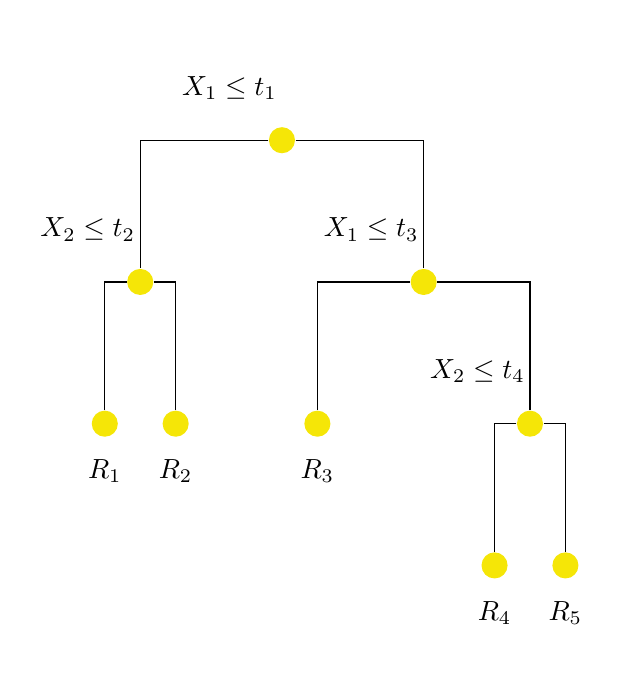
\begin{tikzpicture}
            [scale=.9,auto=center,every node/.style={circle,fill=feadevcolor}]
            
            \node[label=above left: {$X_1 \leq t_1$}] (a1) at (5,7) {};  
            \node[label=above left: {$X_2 \leq t_2$}] (a2) at (3,5) {}; 
            \node[label=above left: {$X_1 \leq t_3$}] (a3) at (7,5) {};
            \node[label=below:{$R_1$}] (a4) at (2.5,3){};
            \node[label=below:{$R_2$}] (a5) at (3.5,3){};
            \node[label=below:{$R_3$}] (a6) at (5.5,3){};
            \node[label=above left:{$X_2 \leq t_4$}] (a7) at (8.5,3){};
            \node[label=below:{$R_4$}] (a8) at (8, 1){};
            \node[label=below:{$R_5$}] (a9) at (9, 1){};
            \draw (a1) -| (a2);
            \draw (a1) -| (a3);
            \draw (a2) -| (a4);
            \draw (a2) -| (a5);
            \draw (a3) -| (a6);
            \draw (a3) -| (a7);
            \draw (a7) -| (a8);
            \draw (a7) -| (a9);
            \end{tikzpicture}
        \column{.3\linewidth}
        \caption{Tree corresponding to the partition in the previous slide.}
    \end{columns}
\end{figure}    
\end{frame}

\subsection{Classification trees}
\begin{frame}{Atributos para classification trees}

    Um dos principais atributos utilizados para definir o corte a ser feito em um modelo de classificação é a \textbf{Entropia de Shannon}, que mede o grau de inversibilidade ($G_i$) de um sistema. Na figura abaixo, o primeiro sistema tem um $G_i$ grande, visto que a quantidade de informação necessária para descrever com precisão qual a cor da bolinha a ser retirada é zero.
    
    \begin{figure}
        \centering
        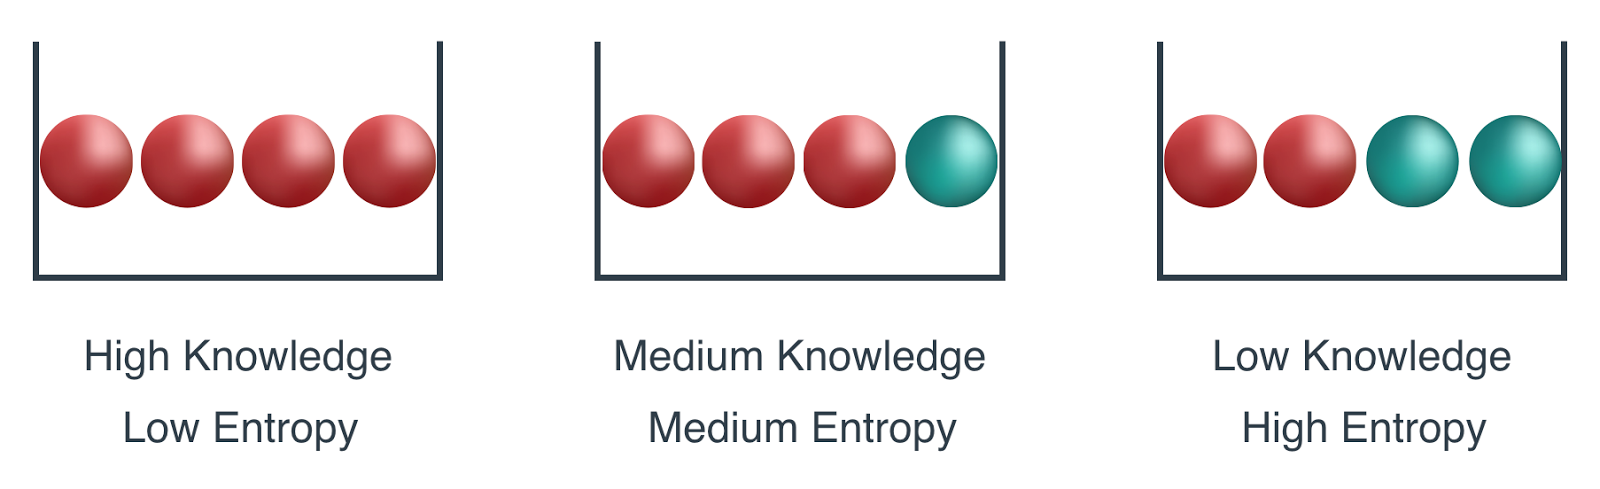
\includegraphics[height=3cm]{pic/entropy.png}
        
    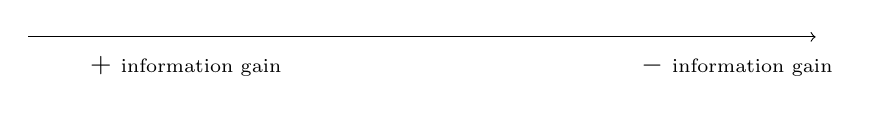
\begin{tikzpicture}
    \node[label=below: {$+$ \scriptsize{information gain}}] at (2,0){};
    \node[label=below: {$-$ \scriptsize{information gain}}] at (9,0){};
    
    \begin{scope}[->]
        \draw[arrowstart] (0,0) -- +(10,0);
    \end{scope}
    \end{tikzpicture}
    
    \caption{Representação da entropia}
    \end{figure}

\end{frame}

\begin{frame}{Entropia de Shannon}
    A equação matemática que define entropia é
    
    \begin{equation}
        Entropy = - \sum_{i=1}^n p_i \log{2p_i},
    \end{equation}
    onde há $n$ classes, e $p_i$ é a probabilidade de um objeto da classe $i$ "aparecer". Usamos $\log{2}$ pois estamos tratando, intrisicamente, de \textit{bits}.
    
    \begin{center}
        \textcolor{feadevcolor}{\textbf{Exemplo}}
    \end{center}
    
    \begin{columns}
        \column{.5\linewidth}
    
            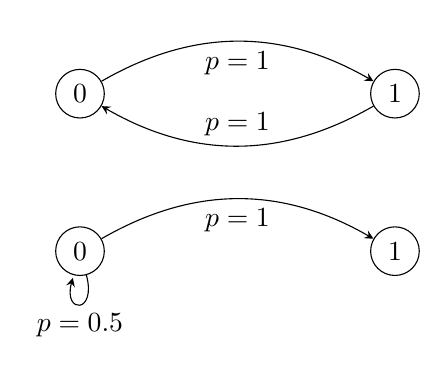
\begin{tikzpicture}[>=stealth,node distance=2.7cm,auto]
            
            \node[anchor=north east,circle, draw] (a1) at (1,3){0};
            \node[anchor=north east,circle, draw] (a2) at (5,3){1};
            
            \node[anchor=north east,circle, draw] (a3) at (1,1){0};
            \node[anchor=north east,circle, draw] (a4) at (5,1){1};
            
            \path[->]
                (a1) edge[swap, bend left] node {$p=1$} (a2)
                (a2) edge[swap, bend left] node {$p=1$} (a1)
                (a3) edge[swap, bend left] node {$p=1$} (a4)
                (a3) edge[swap, loop below] node {$p=0.5$} (a3);
            \end{tikzpicture}
    \column{.5\linewidth}
    \begin{multline*}
        H(S_1) = -(1 \log_21 +\\
        1 \log_21) = 0
    \end{multline*}
    \begin{multline*}
        H(S_2) = -(0.5 \log_2 0.5 +\\
        \hspace{0.1\textwidth} 0.5 \log_2 0.5) = 1
    \end{multline*}
    \end{columns}

\end{frame}

\begin{frame}{Gini Impurity}
Outro atributo para cortes é o de Gini. Para entender, suponha o seguinte:
\begin{enumerate}
    \item Escolhemos aleatoriamente um ponto de dados em nosso conjunto de dados e, em seguida,
    \item Classificamos aleatoriamente de acordo com a distribuição da classe no conjunto de dado;
    \item A probabilidade dessas observações terem classificação diferentes, é a impureza de Gini.
    
    O índice de Gini é definido por
    \begin{equation}
        G = \sum_{k=1}^K \hat{p}_{mk}(1-\hat{p}_{mk}),
    \end{equation}
    onde $\hat{p}_{mk}$ é a proporção de observações classificadas como sendo da categoria $m$ que caem na região $K$. 
\end{enumerate}
    
\end{frame}

\begin{frame}{Exemplo de Gini Impurity}
Leve em consideração um dataset binário, em que temos que classificar data points como azul ou verde. Qual a probabilidade dessas observações serem classificadas incorretamente?

    \begin{table}[h!]
    \centering
    \begin{tabular}{l c}
        \thead{Event} &  \thead{Probability}\\
         \hline
        Pick Blue, Classify Blue \checkmark & 25\%\\
        Pick Blue, Classify Green \faTimes & 25\%\\
        Pick Green, Classify Green \faTimes & 25\%\\
        Pick Green, Classify Blue \checkmark & 25\%\\
    \end{tabular}
    \caption{Descrição probabilística de um dataset fictício.}
    \label{table:1}
    
    \end{table}
    
    O cálculo da impureza de Gini nos dá a resposta,
    
    \begin{align*}
        G & = p(1) \times (1-p(1)) + p(2) \times (1-p(2))\\
        & = 0.5 \times (1-0.5) + 0.5 \times (1-0.5)\\
        & = \textbf{0.5}
    \end{align*}
        
\end{frame}
\begin{frame}{Análise dos atributos de impureza}
\begin{figure}
    \centering
    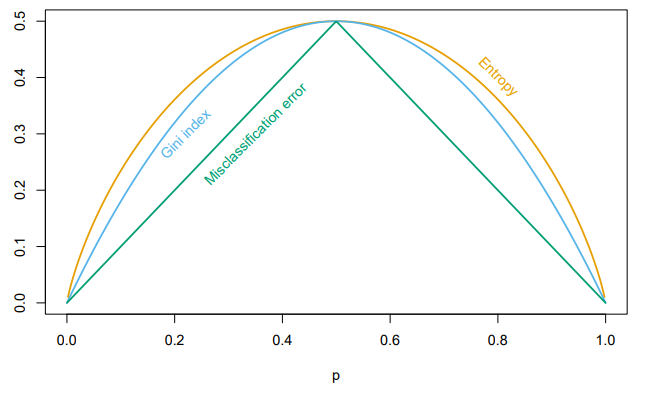
\includegraphics[height=7cm]{pic/gini_entropy_miserror.png}
    \caption{Medida de impureza para uma caso de classificação binária}
\end{figure}
\end{frame}

\section{Códigos em Python}

\begin{frame}[fragile]
\frametitle{Aplicação em Python}
\begin{minted}[linenos]{python}
# Load do dataset iris
data = load_iris()
X = data.data
y = data.target

# Separar em dados de treino e teste
X_train, X_test, y_train, y_test = train_test_split(X, y,
                            random_state=36, test_size=0.25)

# Instanciar, treinar e ver a acurácia do modelo
clf_gini = DecisionTreeClassifier(min_samples_leaf=3,
                    criterion='gini', random_state=34)

clf_gini.fit(X_train, y_train)
y_pred_clfg = clf_gini.predict(X_test)
print("Acc with Gini:" ,accuracy_score(y_test, y_pred_clfg))
\end{minted}
\end{frame}

\begin{frame}{Tree}
\begin{figure}
\centering
    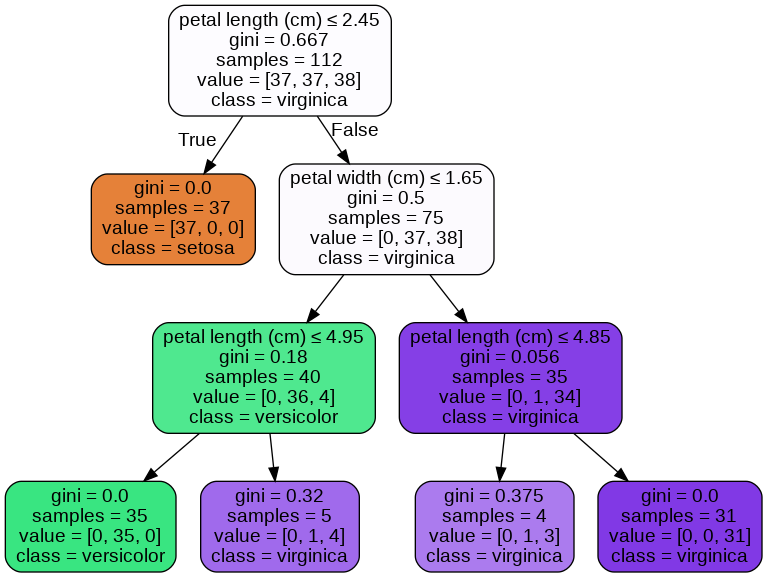
\includegraphics[height=7cm]{pic/decision_tree_graphivz.png}
    \caption{Tree of Decision Tree Classifier model}
\end{figure}
\end{frame}

\begin{frame}{Decision Boundary}
\begin{figure}
    \centering
    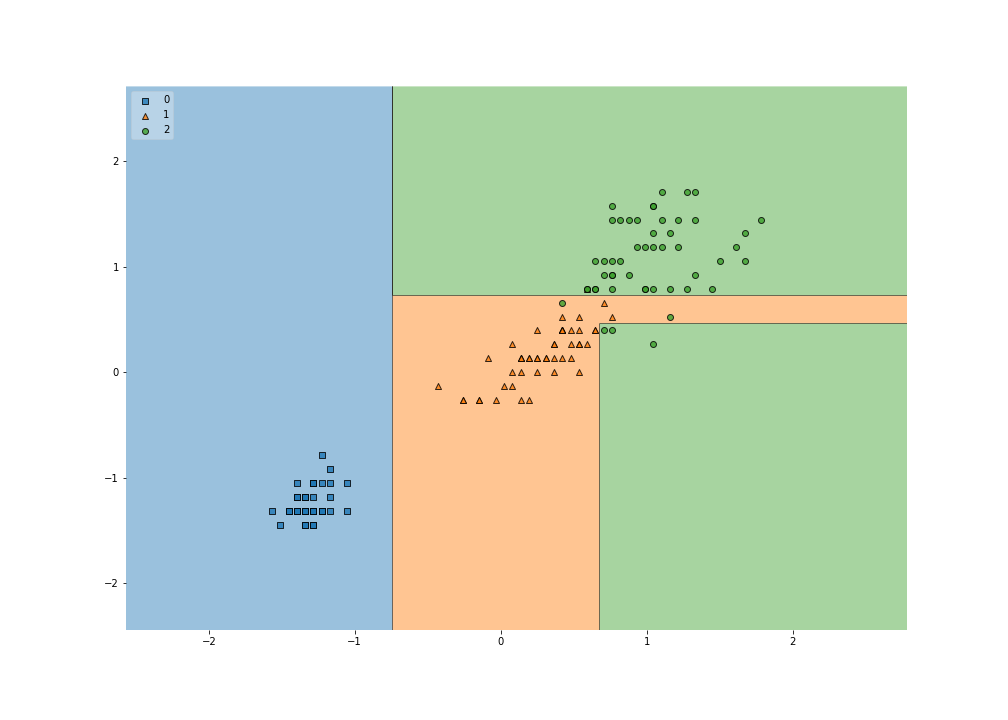
\includegraphics[height=7cm]{pic/decision_boundary.png}
    \caption{Decision boundary of iris dataset}
\end{figure}    
\end{frame}

\section{}
\begin{frame}{Frame Title}

\listoffigures    
\end{frame}
\end{document}

